\documentclass[11pt,a4paper]{report}	% report - article
\usepackage{graphicx}
\usepackage{fancyhdr} 
\usepackage{fancybox} 
\usepackage{psfrag}
\usepackage{boxedminipage} 
\usepackage{epsfig}
\usepackage{amsmath}
\usepackage[ngerman]{babel}
\usepackage[T1]{fontenc}	%fr Sonderzeichen s. latin1
\usepackage[latin1]{inputenc}   %fr Umlaute & scharfes s
\usepackage{times}
\usepackage{float}
\usepackage{amsmath,amssymb}
\usepackage[dvips, a4paper, raiselinks, breaklinks, colorlinks, bookmarks, bookmarksnumbered,citecolor = black, linkcolor = black]{hyperref}
\usepackage{zardozDipl} 
\usepackage{url}







%
%
%\fancypagestyle{plain}{%
%    \lhead{LaTeX - TeXnicCenter} %left head
%    \rhead{Vorlage V2.0} % right head
%    \lfoot{Institut fr Robotik}
%    \rfoot{\thepage}
%    \cfoot{}		%keine Seitenangabe zustzlich in der Mitte !!!
%    \renewcommand{\headrulewidth}{0.4pt}
%    \renewcommand{\footrulewidth}{0.4pt}
%}
%
\pagestyle{plain}
%
\pagenumbering{arabic}
%
%\newtheorem{Aufgabe}{Aufgabe}[section]
%\newtheorem{Hinweis}{Hinweis}[section]
%
%
%\renewcommand{\chaptermark}[1]{}%   %shows chapter left header
%     
\renewcommand{\sectionmark}[1]{\markright{\thesection\ #1}{}}
%
\newcommand{\qu}{\symbol{94}}  %"^" !!!
\newcommand{\MS}{MatLab/SimuLink }
%
%--------------------------------------------------
%
\setlength{\parindent}{0mm}




\setcounter{section}{0}

\begin{document}

		%\textwidth 16cm
%\textheight 25cm
%\topmargin 3.2cm
%\oddsidemargin 0mm
%\parindent 0pt

\thispagestyle{empty}

% Verschiebung der Coverpage in X und Y. Einheit in cm.
\def\DELTAX{0.8}
\def\DELTAY{4.0}


% -------- only change entries beginning here ----------------------------
%
% enter the title of the thesis
%
\def\title{Leonardo da Vinci Program }
%
% choose type of work: 0 ... Dissertation
%                      1 ... Diplomarbeit
%                      2 ... Masterarbeit
\def\type{1}
%
%
% enter name of degree, see examples below
%
\def\degree{Internship}
%\def\degree{Diplomingenieurin}
%\def\degree{Master of Science}
%\def\degree{Doktor}
%\def\degree{Doktorin}

% enter the study (Studienrichtung)
% e.g. Diplomstudium:
%\def\study{Technische Mathematik}
% e.g. Masterstudium:
% \def\study{Industriemathematik}
% e.g. Doktorratsstudium
%\def\study{Technischen Wissenschaften}
%\def\study{Naturwissenschaften}
\def\study{Mechatronik}


% enter the name of the student
%
\def\name{Aaron Martinez Romero}
%
%
% enter the name of the institute
% e.g.
% \def\institute{Institut f\"ur Industriemathematik}
%
\def\institute{Institut f\"ur Robotik}
%
%
% enter the name of the supervisor (who is also the first referee)
% was also the supervisor, do so by choosing the line with (Betreuung)
%
\def\firstreferee{o. Univ.--Prof.\ Dr.--Ing.\ habil.\ Hartmut\ Bremer}
%
%
% in case of a second referee: uncomment the following line and enter the name
%
%\def\secondreferee{Prof.\ Dr.--Ing.\ habil.\ Dr. h.c. i.R.\ Max \ Muster}
%
%
% if there has been assistance by further people uncomment the following line
% and enter the name(s). if there are several assistants speerate the names by \\
%
 \def\assist{Name of assistant}
%\def\assist{Name of first assistant \\ Name of second assistant}
%
%
% enter month year
\def\date{March, 2011}
%
%
% the vertival alignment heavily depends on the length of the title if there are
% one or two supervisors or referees. whereever indicated as a question
%      more space ???
% below you might add additional space via (several) \medskip or \bigskip.
% do not change anything else
% -------------------------------------------------------------------------------
%
\def\ifundefined#1{\expandafter\ifx\csname#1\endcsname\relax}
%
\unitlength 1cm



\sffamily
\begin{picture}(0,0)(\DELTAX,\DELTAY)
\put(-2.6,5){\color{blue}\rule{25cm}{2.6cm}}
\put(10.8,5.15){\small UNIVERSIT\"AT}
\put(13.62,5.15){\small LINZ}
\put(10.8,5.5){\small JOHANNES}
\put(13,5.5){\small KEPLER}
\put(15,5.15){\Huge JKU}
\put(14.75,5.15){\line(0,1){.6}}
%\put(9.7,5.6){
\includegraphics[width=9mm]{img/wap_small.png}}
%\put(0,1){
\includegraphics[width=3cm]{img/tnf.png}}
\put(3.2,1.4){\scriptsize Technisch-Naturwissenschaftliche}
\put(3.2,1.05){\scriptsize Fakult\"at}
\end{picture}
%
\vspace{\DELTAY cm}

\begin{center}
{\LARGE\bfseries\title}
\bigskip\bigskip\bigskip\par
{\Large\ifcase\type DISSERTATION\or DIPLOMARBEIT\or MASTERARBEIT\fi}
\bigskip\par
zur Erlangung des akademischen Grades
\bigskip\smallskip\par
{\Large\degree}
\bigskip\par
im \ifcase\type Doktoratsstudium der\or Diplomstudium\or Masterstudium\fi
\bigskip\smallskip\par
{\Large\study}
\end{center}
%
% more space ???
%\bigskip
\bigskip\bigskip\bigskip\par
Eingereicht von:
\smallskip\par
{\large\name}
\medskip\bigskip\par
Angefertigt am:
\smallskip\par
{\large\institute}
\medskip\bigskip\par
Beurteilung:
\smallskip\par
{\large\firstreferee}
\ifundefined{secondreferee}\else {\large (Betreuung)}
\smallskip\par
{\large\secondreferee}\fi
\ifundefined{assist}\else
\medskip\bigskip\par
Mitwirkung:
\smallskip\par
{\large\assist}
\fi
%
% more space ???
%\bigskip
\bigskip\bigskip\bigskip\par
{\large Linz, \date}

\rmfamily 
	

		\pagestyle{zardoz}
		
		\textheight 24cm
		\textwidth 16cm
		\oddsidemargin 8mm
		\topmargin -15mm
		\headheight 1cm
		\headsep 1cm


		\pagenumbering{roman}
		\setcounter{page}{1}
		\tableofcontents																																   

		%----------------------------------------------------------------------------------
		%										 L I S T  O F  F I G U R E S                                   
		%----------------------------------------------------------------------------------
%		\listoffigures																																		 
%		\addcontentsline{toc}{chapter}{List of Figures} 																	 

		%----------------------------------------------------------------------------------
		%										 L I S T  O F  T A B L E S                                     
		%----------------------------------------------------------------------------------
%		\listoftables																																		   
%		\addcontentsline{toc}{chapter}{List of Tables}																		 

		%----------------------------------------------------------------------------------
		%										 C H A P T E R S                                               
		%----------------------------------------------------------------------------------
		\pagebreak
		\pagenumbering{arabic}
    \setcounter{page}{1}																										
    	\chapter*{TODO}
		\begin{verbatim}
		* poner esquema de la placa de alimentacion del kinect, switch, conversor
		* tutorial to do a new model using google SketchUP
		* tutorial to make a new msgs and srv
		* explain the teleop_joy and teleop_key
		* explain the launch file
		* explain the server and client
		* make a diagram of all the system
		* make a class diagram
		* instalation driver canbus,
		* scan manual for the configuration of 424 to 232 converser
		* create a CD with all the code and models and documents
		* explicar AMCL -> http://www.ros.org/wiki/amcl
		* 
		\end{verbatim}    
    
    		\chapter{Install ROS in Ubuntu}

\section{Configure your Ubuntu repositories:}

Configure your Ubuntu repositories to allow {\bfseries restricted, universe, multiverse}. You can follow the Ubuntu guide ( https://help.ubuntu.com/community/Repositories/Ubuntu ) for instructions on doing this.

\section{Setup your sources.list:}


Setup your sources.list file to accept Debian packages from the ROS server.  
\newline

{\hspace{2em}\bfseries Ubuntu 9.04 (Jaunty)}

\hspace{4em}
sudo sh -c 'echo "deb http://code.ros.org/packages/ros/ubuntu jaunty main" > /etc/apt/sources.list.d/ros-latest.list'
\newline
 
{\hspace{2em}\bfseries Ubuntu 9.10 (Karmic)}

\hspace{4em}
sudo sh -c 'echo "deb http://code.ros.org/packages/ros/ubuntu karmic main" > /etc/apt/sources.list.d/ros-latest.list'
\newline

{\hspace{2em}\bfseries Ubuntu 10.04 (Lucid)}

\hspace{4em}
sudo sh -c 'echo "deb http://code.ros.org/packages/ros/ubuntu lucid main" > /etc/apt/sources.list.d/ros-latest.list'
\newline

{\hspace{2em}\bfseries Ubuntu 10.10 (Maverick)}

\hspace{4em}
sudo sh -c 'echo "deb http://code.ros.org/packages/ros/ubuntu maverick main" > /etc/apt/sources.list.d/ros-latest.list'
\newline

{\bfseries * (In this tutorial we will use the Ubuntu 10.10)}


\section{Set up your keys:}

\hspace{2em}wget http://code.ros.org/packages/ros.key -O - | sudo apt-key add -
\newline

\section{Installation}

Make sure you have re-indexed the ROS.org server:

    \hspace{2em} sudo apt-get update
\newline

Choose your preferred install:

{\hspace{2em}\bfseries ROS only:}

\hspace{4em}
sudo apt-get install ros-cturtle-ros
\newline


{\hspace{2em}\bfseries Base:} ROS plus robot-generic stacks (e.g. navigation, visualization)

\hspace{4em}
sudo apt-get install ros-cturtle-base
\newline


{\hspace{2em}\bfseries PR2:} ROS plus PR2-specific stacks, including PR2 simulator.

\hspace{4em}
sudo apt-get install ros-cturtle-pr2
\newline


{\hspace{2em}\bfseries PR2 All:} ROS plus PR2 and bleeding edge research/experimental stacks.

\hspace{4em}
sudo apt-get install ros-cturtle-pr2all
\newline

{\hspace{2em}\bfseries Stack-specific:} You can also install a specific ROS stack (replace underscores with dashes of the stack name):

\hspace{4em}
sudo apt-get install ros-cturtle-STACK

\hspace{4em}
sudo apt-get install ros-cturtle-slam-gmapping


\section{Environment setup}

It's convenient if the ROS environment variables are automatically added to your bash session every time a new shell is launched:
\newline

\hspace{2em} echo "source /opt/ros/cturtle/setup.bash" >> ~/.bashrc

\hspace{2em} . ~/.bashrc
\newline

If you just want to change the environment of your current shell, you can type:
\newline

\hspace{2em} source /opt/ros/cturtle/setup.bash
\newline

And with all this, the system must be installed.



		\chapter{Install Development Tools}
In the project we are using:

\hspace{2em} {\bfseries Code::Blocks}

\hspace{2em} {\bfseries  Kile}

\section{Script to install from Code::Blocks from SVN}

\begin{verbatim}
#! /bin/bash

cd

mkdir dev # creamos una carpeta para descargar todo y compilar todo

cd dev

mkdir codeblocks

cd codeblocks

sudo apt-get install build-essential libgtk2.0-dev libwxgtk2.8-0 
libwxgtk2.8-dev wx-common subversion autoconf automake libtool 
gobjc++ cmake-curses-gui

svn checkout svn://svn.berlios.de/codeblocks/trunk

cd trunk

export ACLOCAL_FLAGS="-I ‘wx-config --prefix‘/share/aclocal"

./bootstrap

./configure --with-contrib-plugins=all

make

sudo make install

echo /usr/local/lib | sudo tee -a /etc/ld.so.conf

sudo ldconfig

\end{verbatim}


\section{Install Kile from the repositories}

Only we need execute the next comand:

\hspace{2em} sudo apt-get install kile
		\chapter{Download and compile the stack}

In this project we are created a Stack to ROS (Robot Operating System). This stack contain all the code, drivers and nodes developed in the peoject.
The code is hosted in github (http://www.github.com) in the next url


\begin{verbatim}
    cd
    cd dev
    git clone git://github.com/AaronMR/JKU_Robotic_Stack.git
\end{verbatim}


now is necessary update your ROS\_PACKAGE\_PATH environment variable

\begin{verbatim}
    export ROS_PACKAGE_PATH=~/dev/JKU_Robotic_Stack:$ROS_PACKAGE_PATH
\end{verbatim}


		%\chapter{Install ROS in Ubuntu}

\section{Configure your Ubuntu repositories:}

Configure your Ubuntu repositories to allow "restricted," "universe," and "multiverse." You can follow the Ubuntu guide ( https://help.ubuntu.com/community/Repositories/Ubuntu ) for instructions on doing this.

\section{Setup your sources.list:}


Setup your sources.list file to accept Debian packages from the ROS server.  

Ubuntu 9.04 (Jaunty)

sudo sh -c 'echo "deb http://code.ros.org/packages/ros/ubuntu jaunty main" > /etc/apt/sources.list.d/ros-latest.list'

 

Ubuntu 9.10 (Karmic)

sudo sh -c 'echo "deb http://code.ros.org/packages/ros/ubuntu karmic main" > /etc/apt/sources.list.d/ros-latest.list'

Ubuntu 10.04 (Lucid)

sudo sh -c 'echo "deb http://code.ros.org/packages/ros/ubuntu lucid main" > /etc/apt/sources.list.d/ros-latest.list'

Ubuntu 10.10 (Maverick)

sudo sh -c 'echo "deb http://code.ros.org/packages/ros/ubuntu maverick main" > /etc/apt/sources.list.d/ros-latest.list'

* (In this tutorial we will use the Ubuntu 10.10)


\section{Set up your keys:}

wget http://code.ros.org/packages/ros.key -O - | sudo apt-key add -

\section{Installation}

Make sure you have re-indexed the ROS.org server:

    * sudo apt-get update



Choose your preferred install:

ROS only:

    * sudo apt-get install ros-cturtle-ros



Base: ROS plus robot-generic stacks (e.g. navigation, visualization)

    * sudo apt-get install ros-cturtle-base



PR2: ROS plus PR2-specific stacks, including PR2 simulator.

    * sudo apt-get install ros-cturtle-pr2



PR2 All: ROS plus PR2 and bleeding edge research/experimental stacks.

    * sudo apt-get install ros-cturtle-pr2all



Stack-specific: You can also install a specific ROS stack (replace underscores with dashes of the stack name):

    * sudo apt-get install ros-cturtle-STACK
    * sudo apt-get install ros-cturtle-slam-gmapping

\section{Environment setup}

It's convenient if the ROS environment variables are automatically added to your bash session every time a new shell is launched:

 echo "source /opt/ros/cturtle/setup.bash" >> ~/.bashrc

 . ~/.bashrc

If you just want to change the environment of your current shell, you can type:

 source /opt/ros/cturtle/setup.bash

And with all this, the system must be installed.



		%\chapter{Download and install Code::Blocks}


		%\chapter{Install and configure git}
		%\chapter{Download repositories from AaronMR}
		%\chapter{Direction and velocity from the simulator}

linear
x = + es hacia delante
y
z

angular
x
y
z = minus is to right
		%\chapter{ROS tutorials}

\section{Launch simulator with navigation stack}

\begin{verbatim}

Setting up your robot using tf:
http://www.ros.org/wiki/navigation/Tutorials/RobotSetup/TF

urdf:
http://www.ros.org/wiki/urdf
http://www.ros.org/wiki/urdf/Tutorials/Create%20your%20own%20urdf%20file
http://www.ros.org/wiki/urdf/Tutorials/Create%20your%20own%20urdf%20file


:Stack Navigation
http://www.ros.org/wiki/navigation

Install kinect:
http://www.ros.org/wiki/kinect
http://www.ros.org/wiki/kinect/Tutorials/Getting%20Started
http://www.ros.org/wiki/kinect_calibration

gmapping:
http://www.ros.org/wiki/gmapping

Simulating the 2dnav Stack:
http://www.ros.org/wiki/pr2_2dnav_gazebo/Tutorials/Simulating the 2dnav Stack
\end{verbatim}

		%\chapter*{Tutorial 3}

Create a new struct to send and receive from Server and Client.

\section{Client}
\begin{verbatim}

create a new file (process_X.cfg) for the configuration of the process

process(
	name = Process_X
	SHM = SHM_X
	Subscriber = cmd_vel
	Publisher = odom_1
 	Node2RTAI  = posWheels
	RTAI2Node  = posWheels
	IP_RTAI  = 140.78.133.43
	PORT_RTAI  = 1101
)

In the file "AaronMR_Robotic_Stack/Drivers/CB_TCP_RTAI/include/TCP_RTAI/comStruct.h" create a new struct:

  struct posWheels_t
  {
    Point pos_W[4];
  };


In the file "AaronMR_Robotic_Stack/Drivers/CB_TCP_RTAI/include/TCP_RTAI/structType_C.hpp", create a new subclass:

class struct_posWheels : public structType {

public:
    posWheels();
    int serialize(char* data2s);
    int Unserialize(char* data2us);
    void* set_Publisher(char* name);
    void* set_Subscriber(char* name);

    ros::NodeHandle n;
    ros::Publisher posWheels_pub;
    ros::Subscriber posWheels_sub;

    // struct to send and receive
    posWheels_t data2send;
    posWheels_t data2recv;

    geometry_msgs::Point point_msg;
    void cmdCallback(const geometry_msgs::Point &data_);
    bool haveSubscriber;
    bool havePublisher;
    pthread_mutex_t mutex;
    bool canRecv_t;
    bool canSend_t;
    bool canSend();
    bool canRecv();
    int spinOnce();
};


create a new file for the new class, "struct_posWheels.cpp" with the content:

#include "pack2.hpp"
#include "structType_C.hpp"

struct_posWheels::struct_posWheels()
{

}

void struct_posWheels::cmdCallback(const geometry_msgs::Point &data_)
{

}

void* struct_posWheels::set_Subscriber(char* name)
{

}

void* struct_posWheels::set_Publisher(char* name)
{

}

bool struct_posWheels::canSend()
{

}

bool struct_posWheels::canRecv()
{

}

int struct_posWheels::spinOnce()
{

}

int struct_posWheels::serialize(char* data2s)
{

}

int struct_posWheels::Unserialize(char* data2us)
{

}


In the constructor:

struct_posWheels::struct_posWheels()
{

    haveSubscriber  = false;
    havePublisher   = false;
    canRecv_t       = true;
    canSend_t       = true;
    mutex           = PTHREAD_MUTEX_INITIALIZER;

}


Configure the functions to serialize and unserialize:

int struct_posWheels::serialize(char* data2s)
{
   
    unsigned char buf[1024];
    unsigned char magic;
    unsigned int packetsize;
    unsigned int ps2;

    posWheels_t aux;

    aux.pos_W[0].x = 0.0;
    aux.pos_W[0].y = 0.0;
    aux.pos_W[0].z = 0.0;

    aux.pos_W[1].x = 0.0;
    aux.pos_W[1].y = 0.0;
    aux.pos_W[1].z = 0.0;

    aux.pos_W[2].x = 0.0;
    aux.pos_W[2].y = 0.0;
    aux.pos_W[2].z = 0.0;

    aux.pos_W[3].x = 0.0;
    aux.pos_W[3].y = 0.0;
    aux.pos_W[3].z = 0.0;

    packetsize = pack(buf, "CHdddddddddddd",  'A',
					      0,
                                              aux.pos_W[0].x,
                                              aux.pos_W[0].y,
                                              aux.pos_W[0].z,
                                              aux.pos_W[1].x,
                                              aux.pos_W[1].y,
                                              aux.pos_W[1].z,
                                              aux.pos_W[2].x,
                                              aux.pos_W[2].y,
                                              aux.pos_W[2].z,
                                              aux.pos_W[3].x,
                                              aux.pos_W[3].y,
                                              aux.pos_W[3].z);

    packi16(buf+1, packetsize); // store packet size in packet for kicks
    memcpy((unsigned char*)data2s, buf, packetsize);

    return 0;
}

int struct_posWheels::Unserialize(char* data2us)
{

    unsigned char buf[1024];
    unsigned char magic;
    unsigned int ps2;

    memcpy(buf, data2us, 1024);

    posWheels_t aux;

    aux.pos_W[0].x = 0.0;
    aux.pos_W[0].y = 0.0;
    aux.pos_W[0].z = 0.0;

    aux.pos_W[1].x = 0.0;
    aux.pos_W[1].y = 0.0;
    aux.pos_W[1].z = 0.0;

    aux.pos_W[2].x = 0.0;
    aux.pos_W[2].y = 0.0;
    aux.pos_W[2].z = 0.0;

    aux.pos_W[3].x = 0.0;
    aux.pos_W[3].y = 0.0;
    aux.pos_W[3].z = 0.0;

    unpack((unsigned char*)buf, "CHdddddddddddd",&magic,
                                                &ps2,
                                                &aux.pos_W[0].x,
                                                &aux.pos_W[0].y,
                                                &aux.pos_W[0].z,
                                                &aux.pos_W[1].x,
                                                &aux.pos_W[1].y,
                                                &aux.pos_W[1].z,
                                                &aux.pos_W[2].x,
                                                &aux.pos_W[2].y,
                                                &aux.pos_W[2].z,
                                                &aux.pos_W[3].x,
                                                &aux.pos_W[3].y,
                                                &aux.pos_W[3].z);


    return 0;
}


In the file "AaronMR_C.cpp", add the next lines:

// Configure type of struct to send
...
else if(configuration[0].Node2RTAI.compare("posWheels") == 0)
{
  structToSend = new struct_posWheels;
}

// configure type of struct to receive
...
else if(configuration[0].RTAI2Node.compare("posWheels") == 0)
{
  structToRecv = new struct_posWheels;
}

\end{verbatim}

\section{Server}

\begin{verbatim}

Add a new configuration in the file "ServerFile.cfg" for the configuration of the new process

process(
	name = Process_X
	SHM = SHM_X
	Subscriber = cmd_vel
	Publisher = odom_1
 	Node2RTAI  = posWheels
	RTAI2Node  = posWheels
	IP_RTAI  = 140.78.133.43
	PORT_RTAI  = 1101
)

In the file "comStruct.h" add the new struct_posWheels

struct posWheels_t
{
  Point pos_W[4];
}

Create a new class in the structType_S.cpp

    class struct_posWheels : public structType {
    public:
      struct_posWheels();
      char* serialize(char* data2s);
      char* Unserialize(char* data2us);
      void storeData(Joy *joy);
      Joy auxJoy1;

      void iniSHM(int shm_in, int shm_out, char* SHM_name);

      Pose auxPose1;
      int sizeof_Joy;
      bool haveSubscriber;
      bool havePublisher;

      struct posWheels_t *dataIN;
      struct posWheels_t *dataOUT;

    };

Create a new file for the new class, "struct_posWheels.cpp" with the content

#include "AaronMR_S.hpp"
#include "pack2.hpp"
#include <rtai_shm.h>

struct_posWheels::struct_posWheels()
{
   auxSerialize.pos_W[0].x = 0.0;
   auxSerialize.pos_W[0].y = 0.0;
   auxSerialize.pos_W[0].z = 0.0;

   auxSerialize.pos_W[1].x = 0.0;
   auxSerialize.pos_W[1].y = 0.0;
   auxSerialize.pos_W[1].z = 0.0;

   auxSerialize.pos_W[2].x = 0.0;
   auxSerialize.pos_W[2].y = 0.0;
   auxSerialize.pos_W[2].z = 0.0;

   auxSerialize.pos_W[3].x = 0.0;
   auxSerialize.pos_W[3].y = 0.0;
   auxSerialize.pos_W[3].z = 0.0;

   auxUnSerialize.pos_W[0].x = 0.0;
   auxUnSerialize.pos_W[0].y = 0.0;
   auxUnSerialize.pos_W[0].z = 0.0;

   auxUnSerialize.pos_W[1].x = 0.0;
   auxUnSerialize.pos_W[1].y = 0.0;
   auxUnSerialize.pos_W[1].z = 0.0;

   auxUnSerialize.pos_W[2].x = 0.0;
   auxUnSerialize.pos_W[2].y = 0.0;
   auxUnSerialize.pos_W[2].z = 0.0;

   auxUnSerialize.pos_W[3].x = 0.0;
   auxUnSerialize.pos_W[3].y = 0.0;
   auxUnSerialize.pos_W[3].z = 0.0;

}

void struct_posWheels::iniSHM(int shm_in, int shm_out, char* SHM_name)
{
   if (shm_in == 1)
   {
       dataIN = (posWheels_t*)rtai_malloc (nam2num(SHM_name), sizeof(struct posWheels_t)) ;

       dataIN->pos_W[0].x = 0.1;
       dataIN->pos_W[0].y = 0.2;
       dataIN->pos_W[0].z = 0.3;

       dataIN->pos_W[1].x = 0.4;
       dataIN->pos_W[1].y = 0.5;
       dataIN->pos_W[1].z = 0.6;

       dataIN->pos_W[2].x = 0.7;
       dataIN->pos_W[2].y = 0.8;
       dataIN->pos_W[2].z = 0.9;

       dataIN->pos_W[3].x = 0.10;
       dataIN->pos_W[3].y = 0.11;
       dataIN->pos_W[3].z = 0.12;
   }

   if (shm_out == 1)
   {
       dataOUT = (posWheels_t*)rtai_malloc (nam2num(SHM_name), sizeof(struct posWheels_t)) ;

       dataOUT->pos_W[0].x = 1.0;
       dataOUT->pos_W[0].y = 2.0;
       dataOUT->pos_W[0].z = 3.0;

       dataOUT->pos_W[1].x = 4.0;
       dataOUT->pos_W[1].y = 5.0;
       dataOUT->pos_W[1].z = 6.0;

       dataOUT->pos_W[2].x = 7.0;
       dataOUT->pos_W[2].y = 8.0;
       dataOUT->pos_W[2].z = 9.0;

       dataOUT->pos_W[3].x = 10.0;
       dataOUT->pos_W[3].y = 11.0;
       dataOUT->pos_W[3].z = 12.0;
   }
}

char *struct_posWheels::serialize(char* buf3)
{
    unsigned char buf[1024];
    unsigned char magic;
    unsigned int packetsize, ps2;

   auxSerialize.pos_W[0].x = dataOUT->pos_W[0].x;
   auxSerialize.pos_W[0].y = dataOUT->pos_W[0].y;
   auxSerialize.pos_W[0].z = dataOUT->pos_W[0].z;

   auxSerialize.pos_W[1].x = dataOUT->pos_W[1].x;
   auxSerialize.pos_W[1].y = dataOUT->pos_W[1].y;
   auxSerialize.pos_W[1].z = dataOUT->pos_W[1].z;

   auxSerialize.pos_W[2].x = dataOUT->pos_W[2].x;
   auxSerialize.pos_W[2].y = dataOUT->pos_W[2].y;
   auxSerialize.pos_W[2].z = dataOUT->pos_W[2].z;

   auxSerialize.pos_W[3].x = dataOUT->pos_W[3].x;
   auxSerialize.pos_W[3].y = dataOUT->pos_W[3].y;
   auxSerialize.pos_W[3].z = dataOUT->pos_W[3].z;

   packetsize = pack(buf, "CHdddddddddddd", 'A',
                                       0,
                                       auxSerialize.pos_W[0].x,
                                       auxSerialize.pos_W[0].y,
                                       auxSerialize.pos_W[0].z,
                                       auxSerialize.pos_W[1].x,
                                       auxSerialize.pos_W[1].y,
                                       auxSerialize.pos_W[1].z,
                                       auxSerialize.pos_W[2].x,
                                       auxSerialize.pos_W[2].y,
                                       auxSerialize.pos_W[2].z,
                                       auxSerialize.pos_W[3].x,
                                       auxSerialize.pos_W[3].y,
                                       auxSerialize.pos_W[3].z
                                       );

   packi16(buf+1, packetsize); // store packet size in packet for kicks

   memcpy((unsigned char*)buf3, buf, packetsize);

    unpack((unsigned char*)buf3, "CHdddddddddddd",
                                           &magic,
                                           &ps2,
                                           &auxSerialize.pos_W[0].x,
                                           &auxSerialize.pos_W[0].y,
                                           &auxSerialize.pos_W[0].z,
                                           &auxSerialize.pos_W[1].x,
                                           &auxSerialize.pos_W[1].y,
                                           &auxSerialize.pos_W[1].z,
                                           &auxSerialize.pos_W[2].x,
                                           &auxSerialize.pos_W[2].y,
                                           &auxSerialize.pos_W[2].z,
                                           &auxSerialize.pos_W[3].x,
                                           &auxSerialize.pos_W[3].y,
                                           &auxSerialize.pos_W[3].z
                                           );

    printf("posWheels - send: '%c' %hhu %f %f %f %f %f %f %f %f %f %f %f %f\n",
                                           magic,
                                           ps2,
                                           auxSerialize.pos_W[0].x,
                                           auxSerialize.pos_W[0].y,
                                           auxSerialize.pos_W[0].z,
                                           auxSerialize.pos_W[1].x,
                                           auxSerialize.pos_W[1].y,
                                           auxSerialize.pos_W[1].z,
                                           auxSerialize.pos_W[2].x,
                                           auxSerialize.pos_W[2].y,
                                           auxSerialize.pos_W[2].z,
                                           auxSerialize.pos_W[3].x,
                                           auxSerialize.pos_W[3].y,
                                           auxSerialize.pos_W[3].z
                                           );

}

char *struct_posWheels::Unserialize(char* buf3)
{

   unsigned char buf[1024];
    unsigned char magic;
    unsigned int ps2;

   memcpy(buf, buf3, 1024);

    unpack((unsigned char*)buf, "CHdddddddddddd",
                                           &magic,
                                           &ps2,
                                           &auxUnSerialize.pos_W[0].x,
                                           &auxUnSerialize.pos_W[0].y,
                                           &auxUnSerialize.pos_W[0].z,
                                           &auxUnSerialize.pos_W[1].x,
                                           &auxUnSerialize.pos_W[1].y,
                                           &auxUnSerialize.pos_W[1].z,
                                           &auxUnSerialize.pos_W[2].x,
                                           &auxUnSerialize.pos_W[2].y,
                                           &auxUnSerialize.pos_W[2].z,
                                           &auxUnSerialize.pos_W[3].x,
                                           &auxUnSerialize.pos_W[3].y,
                                           &auxUnSerialize.pos_W[3].z
                                           );

    printf("posWheels - recv: '%c' %hhu %f %f %f %f %f %f %f %f %f %f %f %f\n",
                                           magic,
                                           ps2,
                                           auxUnSerialize.pos_W[0].x,
                                           auxUnSerialize.pos_W[0].y,
                                           auxUnSerialize.pos_W[0].z,
                                           auxUnSerialize.pos_W[1].x,
                                           auxUnSerialize.pos_W[1].y,
                                           auxUnSerialize.pos_W[1].z,
                                           auxUnSerialize.pos_W[2].x,
                                           auxUnSerialize.pos_W[2].y,
                                           auxUnSerialize.pos_W[2].z,
                                           auxUnSerialize.pos_W[3].x,
                                           auxUnSerialize.pos_W[3].y,
                                           auxUnSerialize.pos_W[3].z
                                           );

   dataIN->pos_W[0].x = auxUnSerialize.pos_W[0].x;
   dataIN->pos_W[0].y = auxUnSerialize.pos_W[0].y;
   dataIN->pos_W[0].z = auxUnSerialize.pos_W[0].z;

   dataIN->pos_W[1].x = auxUnSerialize.pos_W[1].x;
   dataIN->pos_W[1].y = auxUnSerialize.pos_W[1].y;
   dataIN->pos_W[1].z = auxUnSerialize.pos_W[1].z;

   dataIN->pos_W[2].x = auxUnSerialize.pos_W[2].x;
   dataIN->pos_W[2].y = auxUnSerialize.pos_W[2].y;
   dataIN->pos_W[2].z = auxUnSerialize.pos_W[2].z;

   dataIN->pos_W[3].x = auxUnSerialize.pos_W[3].x;
   dataIN->pos_W[3].y = auxUnSerialize.pos_W[3].y;
   dataIN->pos_W[3].z = auxUnSerialize.pos_W[3].z;

   return NULL;
}


Add the next lines in the "AaronMR_S.cpp" file

// configuration send structure
  ...
  ...
}else if(processThread_2.Node2RTAI.compare("posWheels") == 0){
       //Node2RTAI = 6;
       structToRecv = new struct_posWheels;
       structToRecv->iniSHM(1, 0, (char*)processThread_2.SHM_IN.data());
}

...
...
// configuration recv structure
  ...
  ...
}else if(processThread_2.RTAI2Node.compare("posWheels") == 0){
       //RTAI2Node = 6;
       structToSend = new struct_posWheels;
       structToSend->iniSHM(0,1, (char*)processThread_2.SHM_OUT.data());
}

\end{verbatim}


%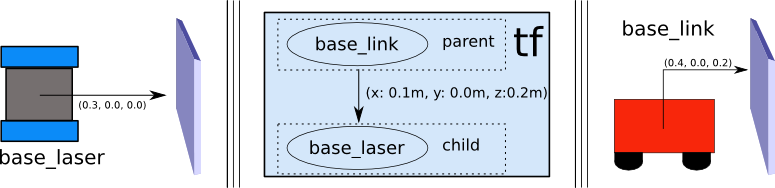
\includegraphics[width=0.5\textwidth,angle=0]{tutorials/tutorial_2/img/tf_robot.png}
		%\chapter*{Tutorial 3}

Create a new struct to send and receive from Server and Client.

\section{Client}
\begin{verbatim}

create a new file (process_X.cfg) for the configuration of the process

process(
	name = Process_X
	SHM = SHM_X
	Subscriber = cmd_vel
	Publisher = odom_1
 	Node2RTAI  = posWheels
	RTAI2Node  = posWheels
	IP_RTAI  = 140.78.133.43
	PORT_RTAI  = 1101
)

In the file "AaronMR_Robotic_Stack/Drivers/CB_TCP_RTAI/include/TCP_RTAI/comStruct.h" create a new struct:

  struct posWheels_t
  {
    Point pos_W[4];
  };


In the file "AaronMR_Robotic_Stack/Drivers/CB_TCP_RTAI/include/TCP_RTAI/structType_C.hpp", create a new subclass:

class struct_posWheels : public structType {

public:
    posWheels();
    int serialize(char* data2s);
    int Unserialize(char* data2us);
    void* set_Publisher(char* name);
    void* set_Subscriber(char* name);

    ros::NodeHandle n;
    ros::Publisher posWheels_pub;
    ros::Subscriber posWheels_sub;

    // struct to send and receive
    posWheels_t data2send;
    posWheels_t data2recv;

    geometry_msgs::Point point_msg;
    void cmdCallback(const geometry_msgs::Point &data_);
    bool haveSubscriber;
    bool havePublisher;
    pthread_mutex_t mutex;
    bool canRecv_t;
    bool canSend_t;
    bool canSend();
    bool canRecv();
    int spinOnce();
};


create a new file for the new class, "struct_posWheels.cpp" with the content:

#include "pack2.hpp"
#include "structType_C.hpp"

struct_posWheels::struct_posWheels()
{

}

void struct_posWheels::cmdCallback(const geometry_msgs::Point &data_)
{

}

void* struct_posWheels::set_Subscriber(char* name)
{

}

void* struct_posWheels::set_Publisher(char* name)
{

}

bool struct_posWheels::canSend()
{

}

bool struct_posWheels::canRecv()
{

}

int struct_posWheels::spinOnce()
{

}

int struct_posWheels::serialize(char* data2s)
{

}

int struct_posWheels::Unserialize(char* data2us)
{

}


In the constructor:

struct_posWheels::struct_posWheels()
{

    haveSubscriber  = false;
    havePublisher   = false;
    canRecv_t       = true;
    canSend_t       = true;
    mutex           = PTHREAD_MUTEX_INITIALIZER;

}


Configure the functions to serialize and unserialize:

int struct_posWheels::serialize(char* data2s)
{
   
    unsigned char buf[1024];
    unsigned char magic;
    unsigned int packetsize;
    unsigned int ps2;

    posWheels_t aux;

    aux.pos_W[0].x = 0.0;
    aux.pos_W[0].y = 0.0;
    aux.pos_W[0].z = 0.0;

    aux.pos_W[1].x = 0.0;
    aux.pos_W[1].y = 0.0;
    aux.pos_W[1].z = 0.0;

    aux.pos_W[2].x = 0.0;
    aux.pos_W[2].y = 0.0;
    aux.pos_W[2].z = 0.0;

    aux.pos_W[3].x = 0.0;
    aux.pos_W[3].y = 0.0;
    aux.pos_W[3].z = 0.0;

    packetsize = pack(buf, "CHdddddddddddd",  'A',
					      0,
                                              aux.pos_W[0].x,
                                              aux.pos_W[0].y,
                                              aux.pos_W[0].z,
                                              aux.pos_W[1].x,
                                              aux.pos_W[1].y,
                                              aux.pos_W[1].z,
                                              aux.pos_W[2].x,
                                              aux.pos_W[2].y,
                                              aux.pos_W[2].z,
                                              aux.pos_W[3].x,
                                              aux.pos_W[3].y,
                                              aux.pos_W[3].z);

    packi16(buf+1, packetsize); // store packet size in packet for kicks
    memcpy((unsigned char*)data2s, buf, packetsize);

    return 0;
}

int struct_posWheels::Unserialize(char* data2us)
{

    unsigned char buf[1024];
    unsigned char magic;
    unsigned int ps2;

    memcpy(buf, data2us, 1024);

    posWheels_t aux;

    aux.pos_W[0].x = 0.0;
    aux.pos_W[0].y = 0.0;
    aux.pos_W[0].z = 0.0;

    aux.pos_W[1].x = 0.0;
    aux.pos_W[1].y = 0.0;
    aux.pos_W[1].z = 0.0;

    aux.pos_W[2].x = 0.0;
    aux.pos_W[2].y = 0.0;
    aux.pos_W[2].z = 0.0;

    aux.pos_W[3].x = 0.0;
    aux.pos_W[3].y = 0.0;
    aux.pos_W[3].z = 0.0;

    unpack((unsigned char*)buf, "CHdddddddddddd",&magic,
                                                &ps2,
                                                &aux.pos_W[0].x,
                                                &aux.pos_W[0].y,
                                                &aux.pos_W[0].z,
                                                &aux.pos_W[1].x,
                                                &aux.pos_W[1].y,
                                                &aux.pos_W[1].z,
                                                &aux.pos_W[2].x,
                                                &aux.pos_W[2].y,
                                                &aux.pos_W[2].z,
                                                &aux.pos_W[3].x,
                                                &aux.pos_W[3].y,
                                                &aux.pos_W[3].z);


    return 0;
}


In the file "AaronMR_C.cpp", add the next lines:

// Configure type of struct to send
...
else if(configuration[0].Node2RTAI.compare("posWheels") == 0)
{
  structToSend = new struct_posWheels;
}

// configure type of struct to receive
...
else if(configuration[0].RTAI2Node.compare("posWheels") == 0)
{
  structToRecv = new struct_posWheels;
}

\end{verbatim}

\section{Server}

\begin{verbatim}

Add a new configuration in the file "ServerFile.cfg" for the configuration of the new process

process(
	name = Process_X
	SHM = SHM_X
	Subscriber = cmd_vel
	Publisher = odom_1
 	Node2RTAI  = posWheels
	RTAI2Node  = posWheels
	IP_RTAI  = 140.78.133.43
	PORT_RTAI  = 1101
)

In the file "comStruct.h" add the new struct_posWheels

struct posWheels_t
{
  Point pos_W[4];
}

Create a new class in the structType_S.cpp

    class struct_posWheels : public structType {
    public:
      struct_posWheels();
      char* serialize(char* data2s);
      char* Unserialize(char* data2us);
      void storeData(Joy *joy);
      Joy auxJoy1;

      void iniSHM(int shm_in, int shm_out, char* SHM_name);

      Pose auxPose1;
      int sizeof_Joy;
      bool haveSubscriber;
      bool havePublisher;

      struct posWheels_t *dataIN;
      struct posWheels_t *dataOUT;

    };

Create a new file for the new class, "struct_posWheels.cpp" with the content

#include "AaronMR_S.hpp"
#include "pack2.hpp"
#include <rtai_shm.h>

struct_posWheels::struct_posWheels()
{
   auxSerialize.pos_W[0].x = 0.0;
   auxSerialize.pos_W[0].y = 0.0;
   auxSerialize.pos_W[0].z = 0.0;

   auxSerialize.pos_W[1].x = 0.0;
   auxSerialize.pos_W[1].y = 0.0;
   auxSerialize.pos_W[1].z = 0.0;

   auxSerialize.pos_W[2].x = 0.0;
   auxSerialize.pos_W[2].y = 0.0;
   auxSerialize.pos_W[2].z = 0.0;

   auxSerialize.pos_W[3].x = 0.0;
   auxSerialize.pos_W[3].y = 0.0;
   auxSerialize.pos_W[3].z = 0.0;

   auxUnSerialize.pos_W[0].x = 0.0;
   auxUnSerialize.pos_W[0].y = 0.0;
   auxUnSerialize.pos_W[0].z = 0.0;

   auxUnSerialize.pos_W[1].x = 0.0;
   auxUnSerialize.pos_W[1].y = 0.0;
   auxUnSerialize.pos_W[1].z = 0.0;

   auxUnSerialize.pos_W[2].x = 0.0;
   auxUnSerialize.pos_W[2].y = 0.0;
   auxUnSerialize.pos_W[2].z = 0.0;

   auxUnSerialize.pos_W[3].x = 0.0;
   auxUnSerialize.pos_W[3].y = 0.0;
   auxUnSerialize.pos_W[3].z = 0.0;

}

void struct_posWheels::iniSHM(int shm_in, int shm_out, char* SHM_name)
{
   if (shm_in == 1)
   {
       dataIN = (posWheels_t*)rtai_malloc (nam2num(SHM_name), sizeof(struct posWheels_t)) ;

       dataIN->pos_W[0].x = 0.1;
       dataIN->pos_W[0].y = 0.2;
       dataIN->pos_W[0].z = 0.3;

       dataIN->pos_W[1].x = 0.4;
       dataIN->pos_W[1].y = 0.5;
       dataIN->pos_W[1].z = 0.6;

       dataIN->pos_W[2].x = 0.7;
       dataIN->pos_W[2].y = 0.8;
       dataIN->pos_W[2].z = 0.9;

       dataIN->pos_W[3].x = 0.10;
       dataIN->pos_W[3].y = 0.11;
       dataIN->pos_W[3].z = 0.12;
   }

   if (shm_out == 1)
   {
       dataOUT = (posWheels_t*)rtai_malloc (nam2num(SHM_name), sizeof(struct posWheels_t)) ;

       dataOUT->pos_W[0].x = 1.0;
       dataOUT->pos_W[0].y = 2.0;
       dataOUT->pos_W[0].z = 3.0;

       dataOUT->pos_W[1].x = 4.0;
       dataOUT->pos_W[1].y = 5.0;
       dataOUT->pos_W[1].z = 6.0;

       dataOUT->pos_W[2].x = 7.0;
       dataOUT->pos_W[2].y = 8.0;
       dataOUT->pos_W[2].z = 9.0;

       dataOUT->pos_W[3].x = 10.0;
       dataOUT->pos_W[3].y = 11.0;
       dataOUT->pos_W[3].z = 12.0;
   }
}

char *struct_posWheels::serialize(char* buf3)
{
    unsigned char buf[1024];
    unsigned char magic;
    unsigned int packetsize, ps2;

   auxSerialize.pos_W[0].x = dataOUT->pos_W[0].x;
   auxSerialize.pos_W[0].y = dataOUT->pos_W[0].y;
   auxSerialize.pos_W[0].z = dataOUT->pos_W[0].z;

   auxSerialize.pos_W[1].x = dataOUT->pos_W[1].x;
   auxSerialize.pos_W[1].y = dataOUT->pos_W[1].y;
   auxSerialize.pos_W[1].z = dataOUT->pos_W[1].z;

   auxSerialize.pos_W[2].x = dataOUT->pos_W[2].x;
   auxSerialize.pos_W[2].y = dataOUT->pos_W[2].y;
   auxSerialize.pos_W[2].z = dataOUT->pos_W[2].z;

   auxSerialize.pos_W[3].x = dataOUT->pos_W[3].x;
   auxSerialize.pos_W[3].y = dataOUT->pos_W[3].y;
   auxSerialize.pos_W[3].z = dataOUT->pos_W[3].z;

   packetsize = pack(buf, "CHdddddddddddd", 'A',
                                       0,
                                       auxSerialize.pos_W[0].x,
                                       auxSerialize.pos_W[0].y,
                                       auxSerialize.pos_W[0].z,
                                       auxSerialize.pos_W[1].x,
                                       auxSerialize.pos_W[1].y,
                                       auxSerialize.pos_W[1].z,
                                       auxSerialize.pos_W[2].x,
                                       auxSerialize.pos_W[2].y,
                                       auxSerialize.pos_W[2].z,
                                       auxSerialize.pos_W[3].x,
                                       auxSerialize.pos_W[3].y,
                                       auxSerialize.pos_W[3].z
                                       );

   packi16(buf+1, packetsize); // store packet size in packet for kicks

   memcpy((unsigned char*)buf3, buf, packetsize);

    unpack((unsigned char*)buf3, "CHdddddddddddd",
                                           &magic,
                                           &ps2,
                                           &auxSerialize.pos_W[0].x,
                                           &auxSerialize.pos_W[0].y,
                                           &auxSerialize.pos_W[0].z,
                                           &auxSerialize.pos_W[1].x,
                                           &auxSerialize.pos_W[1].y,
                                           &auxSerialize.pos_W[1].z,
                                           &auxSerialize.pos_W[2].x,
                                           &auxSerialize.pos_W[2].y,
                                           &auxSerialize.pos_W[2].z,
                                           &auxSerialize.pos_W[3].x,
                                           &auxSerialize.pos_W[3].y,
                                           &auxSerialize.pos_W[3].z
                                           );

    printf("posWheels - send: '%c' %hhu %f %f %f %f %f %f %f %f %f %f %f %f\n",
                                           magic,
                                           ps2,
                                           auxSerialize.pos_W[0].x,
                                           auxSerialize.pos_W[0].y,
                                           auxSerialize.pos_W[0].z,
                                           auxSerialize.pos_W[1].x,
                                           auxSerialize.pos_W[1].y,
                                           auxSerialize.pos_W[1].z,
                                           auxSerialize.pos_W[2].x,
                                           auxSerialize.pos_W[2].y,
                                           auxSerialize.pos_W[2].z,
                                           auxSerialize.pos_W[3].x,
                                           auxSerialize.pos_W[3].y,
                                           auxSerialize.pos_W[3].z
                                           );

}

char *struct_posWheels::Unserialize(char* buf3)
{

   unsigned char buf[1024];
    unsigned char magic;
    unsigned int ps2;

   memcpy(buf, buf3, 1024);

    unpack((unsigned char*)buf, "CHdddddddddddd",
                                           &magic,
                                           &ps2,
                                           &auxUnSerialize.pos_W[0].x,
                                           &auxUnSerialize.pos_W[0].y,
                                           &auxUnSerialize.pos_W[0].z,
                                           &auxUnSerialize.pos_W[1].x,
                                           &auxUnSerialize.pos_W[1].y,
                                           &auxUnSerialize.pos_W[1].z,
                                           &auxUnSerialize.pos_W[2].x,
                                           &auxUnSerialize.pos_W[2].y,
                                           &auxUnSerialize.pos_W[2].z,
                                           &auxUnSerialize.pos_W[3].x,
                                           &auxUnSerialize.pos_W[3].y,
                                           &auxUnSerialize.pos_W[3].z
                                           );

    printf("posWheels - recv: '%c' %hhu %f %f %f %f %f %f %f %f %f %f %f %f\n",
                                           magic,
                                           ps2,
                                           auxUnSerialize.pos_W[0].x,
                                           auxUnSerialize.pos_W[0].y,
                                           auxUnSerialize.pos_W[0].z,
                                           auxUnSerialize.pos_W[1].x,
                                           auxUnSerialize.pos_W[1].y,
                                           auxUnSerialize.pos_W[1].z,
                                           auxUnSerialize.pos_W[2].x,
                                           auxUnSerialize.pos_W[2].y,
                                           auxUnSerialize.pos_W[2].z,
                                           auxUnSerialize.pos_W[3].x,
                                           auxUnSerialize.pos_W[3].y,
                                           auxUnSerialize.pos_W[3].z
                                           );

   dataIN->pos_W[0].x = auxUnSerialize.pos_W[0].x;
   dataIN->pos_W[0].y = auxUnSerialize.pos_W[0].y;
   dataIN->pos_W[0].z = auxUnSerialize.pos_W[0].z;

   dataIN->pos_W[1].x = auxUnSerialize.pos_W[1].x;
   dataIN->pos_W[1].y = auxUnSerialize.pos_W[1].y;
   dataIN->pos_W[1].z = auxUnSerialize.pos_W[1].z;

   dataIN->pos_W[2].x = auxUnSerialize.pos_W[2].x;
   dataIN->pos_W[2].y = auxUnSerialize.pos_W[2].y;
   dataIN->pos_W[2].z = auxUnSerialize.pos_W[2].z;

   dataIN->pos_W[3].x = auxUnSerialize.pos_W[3].x;
   dataIN->pos_W[3].y = auxUnSerialize.pos_W[3].y;
   dataIN->pos_W[3].z = auxUnSerialize.pos_W[3].z;

   return NULL;
}


Add the next lines in the "AaronMR_S.cpp" file

// configuration send structure
  ...
  ...
}else if(processThread_2.Node2RTAI.compare("posWheels") == 0){
       //Node2RTAI = 6;
       structToRecv = new struct_posWheels;
       structToRecv->iniSHM(1, 0, (char*)processThread_2.SHM_IN.data());
}

...
...
// configuration recv structure
  ...
  ...
}else if(processThread_2.RTAI2Node.compare("posWheels") == 0){
       //RTAI2Node = 6;
       structToSend = new struct_posWheels;
       structToSend->iniSHM(0,1, (char*)processThread_2.SHM_OUT.data());
}

\end{verbatim}


%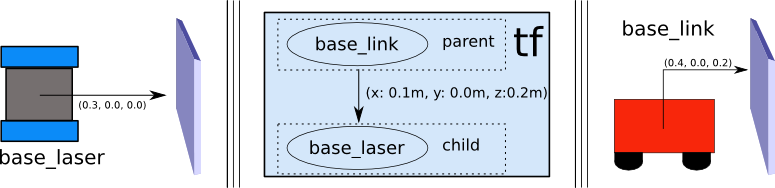
\includegraphics[width=0.5\textwidth,angle=0]{tutorials/tutorial_2/img/tf_robot.png}
		%\include{Navigation}
		%\chapter*{Tutorial 3}

Create a new struct to send and receive from Server and Client.

\section{Client}
\begin{verbatim}

create a new file (process_X.cfg) for the configuration of the process

process(
	name = Process_X
	SHM = SHM_X
	Subscriber = cmd_vel
	Publisher = odom_1
 	Node2RTAI  = posWheels
	RTAI2Node  = posWheels
	IP_RTAI  = 140.78.133.43
	PORT_RTAI  = 1101
)

In the file "AaronMR_Robotic_Stack/Drivers/CB_TCP_RTAI/include/TCP_RTAI/comStruct.h" create a new struct:

  struct posWheels_t
  {
    Point pos_W[4];
  };


In the file "AaronMR_Robotic_Stack/Drivers/CB_TCP_RTAI/include/TCP_RTAI/structType_C.hpp", create a new subclass:

class struct_posWheels : public structType {

public:
    posWheels();
    int serialize(char* data2s);
    int Unserialize(char* data2us);
    void* set_Publisher(char* name);
    void* set_Subscriber(char* name);

    ros::NodeHandle n;
    ros::Publisher posWheels_pub;
    ros::Subscriber posWheels_sub;

    // struct to send and receive
    posWheels_t data2send;
    posWheels_t data2recv;

    geometry_msgs::Point point_msg;
    void cmdCallback(const geometry_msgs::Point &data_);
    bool haveSubscriber;
    bool havePublisher;
    pthread_mutex_t mutex;
    bool canRecv_t;
    bool canSend_t;
    bool canSend();
    bool canRecv();
    int spinOnce();
};


create a new file for the new class, "struct_posWheels.cpp" with the content:

#include "pack2.hpp"
#include "structType_C.hpp"

struct_posWheels::struct_posWheels()
{

}

void struct_posWheels::cmdCallback(const geometry_msgs::Point &data_)
{

}

void* struct_posWheels::set_Subscriber(char* name)
{

}

void* struct_posWheels::set_Publisher(char* name)
{

}

bool struct_posWheels::canSend()
{

}

bool struct_posWheels::canRecv()
{

}

int struct_posWheels::spinOnce()
{

}

int struct_posWheels::serialize(char* data2s)
{

}

int struct_posWheels::Unserialize(char* data2us)
{

}


In the constructor:

struct_posWheels::struct_posWheels()
{

    haveSubscriber  = false;
    havePublisher   = false;
    canRecv_t       = true;
    canSend_t       = true;
    mutex           = PTHREAD_MUTEX_INITIALIZER;

}


Configure the functions to serialize and unserialize:

int struct_posWheels::serialize(char* data2s)
{
   
    unsigned char buf[1024];
    unsigned char magic;
    unsigned int packetsize;
    unsigned int ps2;

    posWheels_t aux;

    aux.pos_W[0].x = 0.0;
    aux.pos_W[0].y = 0.0;
    aux.pos_W[0].z = 0.0;

    aux.pos_W[1].x = 0.0;
    aux.pos_W[1].y = 0.0;
    aux.pos_W[1].z = 0.0;

    aux.pos_W[2].x = 0.0;
    aux.pos_W[2].y = 0.0;
    aux.pos_W[2].z = 0.0;

    aux.pos_W[3].x = 0.0;
    aux.pos_W[3].y = 0.0;
    aux.pos_W[3].z = 0.0;

    packetsize = pack(buf, "CHdddddddddddd",  'A',
					      0,
                                              aux.pos_W[0].x,
                                              aux.pos_W[0].y,
                                              aux.pos_W[0].z,
                                              aux.pos_W[1].x,
                                              aux.pos_W[1].y,
                                              aux.pos_W[1].z,
                                              aux.pos_W[2].x,
                                              aux.pos_W[2].y,
                                              aux.pos_W[2].z,
                                              aux.pos_W[3].x,
                                              aux.pos_W[3].y,
                                              aux.pos_W[3].z);

    packi16(buf+1, packetsize); // store packet size in packet for kicks
    memcpy((unsigned char*)data2s, buf, packetsize);

    return 0;
}

int struct_posWheels::Unserialize(char* data2us)
{

    unsigned char buf[1024];
    unsigned char magic;
    unsigned int ps2;

    memcpy(buf, data2us, 1024);

    posWheels_t aux;

    aux.pos_W[0].x = 0.0;
    aux.pos_W[0].y = 0.0;
    aux.pos_W[0].z = 0.0;

    aux.pos_W[1].x = 0.0;
    aux.pos_W[1].y = 0.0;
    aux.pos_W[1].z = 0.0;

    aux.pos_W[2].x = 0.0;
    aux.pos_W[2].y = 0.0;
    aux.pos_W[2].z = 0.0;

    aux.pos_W[3].x = 0.0;
    aux.pos_W[3].y = 0.0;
    aux.pos_W[3].z = 0.0;

    unpack((unsigned char*)buf, "CHdddddddddddd",&magic,
                                                &ps2,
                                                &aux.pos_W[0].x,
                                                &aux.pos_W[0].y,
                                                &aux.pos_W[0].z,
                                                &aux.pos_W[1].x,
                                                &aux.pos_W[1].y,
                                                &aux.pos_W[1].z,
                                                &aux.pos_W[2].x,
                                                &aux.pos_W[2].y,
                                                &aux.pos_W[2].z,
                                                &aux.pos_W[3].x,
                                                &aux.pos_W[3].y,
                                                &aux.pos_W[3].z);


    return 0;
}


In the file "AaronMR_C.cpp", add the next lines:

// Configure type of struct to send
...
else if(configuration[0].Node2RTAI.compare("posWheels") == 0)
{
  structToSend = new struct_posWheels;
}

// configure type of struct to receive
...
else if(configuration[0].RTAI2Node.compare("posWheels") == 0)
{
  structToRecv = new struct_posWheels;
}

\end{verbatim}

\section{Server}

\begin{verbatim}

Add a new configuration in the file "ServerFile.cfg" for the configuration of the new process

process(
	name = Process_X
	SHM = SHM_X
	Subscriber = cmd_vel
	Publisher = odom_1
 	Node2RTAI  = posWheels
	RTAI2Node  = posWheels
	IP_RTAI  = 140.78.133.43
	PORT_RTAI  = 1101
)

In the file "comStruct.h" add the new struct_posWheels

struct posWheels_t
{
  Point pos_W[4];
}

Create a new class in the structType_S.cpp

    class struct_posWheels : public structType {
    public:
      struct_posWheels();
      char* serialize(char* data2s);
      char* Unserialize(char* data2us);
      void storeData(Joy *joy);
      Joy auxJoy1;

      void iniSHM(int shm_in, int shm_out, char* SHM_name);

      Pose auxPose1;
      int sizeof_Joy;
      bool haveSubscriber;
      bool havePublisher;

      struct posWheels_t *dataIN;
      struct posWheels_t *dataOUT;

    };

Create a new file for the new class, "struct_posWheels.cpp" with the content

#include "AaronMR_S.hpp"
#include "pack2.hpp"
#include <rtai_shm.h>

struct_posWheels::struct_posWheels()
{
   auxSerialize.pos_W[0].x = 0.0;
   auxSerialize.pos_W[0].y = 0.0;
   auxSerialize.pos_W[0].z = 0.0;

   auxSerialize.pos_W[1].x = 0.0;
   auxSerialize.pos_W[1].y = 0.0;
   auxSerialize.pos_W[1].z = 0.0;

   auxSerialize.pos_W[2].x = 0.0;
   auxSerialize.pos_W[2].y = 0.0;
   auxSerialize.pos_W[2].z = 0.0;

   auxSerialize.pos_W[3].x = 0.0;
   auxSerialize.pos_W[3].y = 0.0;
   auxSerialize.pos_W[3].z = 0.0;

   auxUnSerialize.pos_W[0].x = 0.0;
   auxUnSerialize.pos_W[0].y = 0.0;
   auxUnSerialize.pos_W[0].z = 0.0;

   auxUnSerialize.pos_W[1].x = 0.0;
   auxUnSerialize.pos_W[1].y = 0.0;
   auxUnSerialize.pos_W[1].z = 0.0;

   auxUnSerialize.pos_W[2].x = 0.0;
   auxUnSerialize.pos_W[2].y = 0.0;
   auxUnSerialize.pos_W[2].z = 0.0;

   auxUnSerialize.pos_W[3].x = 0.0;
   auxUnSerialize.pos_W[3].y = 0.0;
   auxUnSerialize.pos_W[3].z = 0.0;

}

void struct_posWheels::iniSHM(int shm_in, int shm_out, char* SHM_name)
{
   if (shm_in == 1)
   {
       dataIN = (posWheels_t*)rtai_malloc (nam2num(SHM_name), sizeof(struct posWheels_t)) ;

       dataIN->pos_W[0].x = 0.1;
       dataIN->pos_W[0].y = 0.2;
       dataIN->pos_W[0].z = 0.3;

       dataIN->pos_W[1].x = 0.4;
       dataIN->pos_W[1].y = 0.5;
       dataIN->pos_W[1].z = 0.6;

       dataIN->pos_W[2].x = 0.7;
       dataIN->pos_W[2].y = 0.8;
       dataIN->pos_W[2].z = 0.9;

       dataIN->pos_W[3].x = 0.10;
       dataIN->pos_W[3].y = 0.11;
       dataIN->pos_W[3].z = 0.12;
   }

   if (shm_out == 1)
   {
       dataOUT = (posWheels_t*)rtai_malloc (nam2num(SHM_name), sizeof(struct posWheels_t)) ;

       dataOUT->pos_W[0].x = 1.0;
       dataOUT->pos_W[0].y = 2.0;
       dataOUT->pos_W[0].z = 3.0;

       dataOUT->pos_W[1].x = 4.0;
       dataOUT->pos_W[1].y = 5.0;
       dataOUT->pos_W[1].z = 6.0;

       dataOUT->pos_W[2].x = 7.0;
       dataOUT->pos_W[2].y = 8.0;
       dataOUT->pos_W[2].z = 9.0;

       dataOUT->pos_W[3].x = 10.0;
       dataOUT->pos_W[3].y = 11.0;
       dataOUT->pos_W[3].z = 12.0;
   }
}

char *struct_posWheels::serialize(char* buf3)
{
    unsigned char buf[1024];
    unsigned char magic;
    unsigned int packetsize, ps2;

   auxSerialize.pos_W[0].x = dataOUT->pos_W[0].x;
   auxSerialize.pos_W[0].y = dataOUT->pos_W[0].y;
   auxSerialize.pos_W[0].z = dataOUT->pos_W[0].z;

   auxSerialize.pos_W[1].x = dataOUT->pos_W[1].x;
   auxSerialize.pos_W[1].y = dataOUT->pos_W[1].y;
   auxSerialize.pos_W[1].z = dataOUT->pos_W[1].z;

   auxSerialize.pos_W[2].x = dataOUT->pos_W[2].x;
   auxSerialize.pos_W[2].y = dataOUT->pos_W[2].y;
   auxSerialize.pos_W[2].z = dataOUT->pos_W[2].z;

   auxSerialize.pos_W[3].x = dataOUT->pos_W[3].x;
   auxSerialize.pos_W[3].y = dataOUT->pos_W[3].y;
   auxSerialize.pos_W[3].z = dataOUT->pos_W[3].z;

   packetsize = pack(buf, "CHdddddddddddd", 'A',
                                       0,
                                       auxSerialize.pos_W[0].x,
                                       auxSerialize.pos_W[0].y,
                                       auxSerialize.pos_W[0].z,
                                       auxSerialize.pos_W[1].x,
                                       auxSerialize.pos_W[1].y,
                                       auxSerialize.pos_W[1].z,
                                       auxSerialize.pos_W[2].x,
                                       auxSerialize.pos_W[2].y,
                                       auxSerialize.pos_W[2].z,
                                       auxSerialize.pos_W[3].x,
                                       auxSerialize.pos_W[3].y,
                                       auxSerialize.pos_W[3].z
                                       );

   packi16(buf+1, packetsize); // store packet size in packet for kicks

   memcpy((unsigned char*)buf3, buf, packetsize);

    unpack((unsigned char*)buf3, "CHdddddddddddd",
                                           &magic,
                                           &ps2,
                                           &auxSerialize.pos_W[0].x,
                                           &auxSerialize.pos_W[0].y,
                                           &auxSerialize.pos_W[0].z,
                                           &auxSerialize.pos_W[1].x,
                                           &auxSerialize.pos_W[1].y,
                                           &auxSerialize.pos_W[1].z,
                                           &auxSerialize.pos_W[2].x,
                                           &auxSerialize.pos_W[2].y,
                                           &auxSerialize.pos_W[2].z,
                                           &auxSerialize.pos_W[3].x,
                                           &auxSerialize.pos_W[3].y,
                                           &auxSerialize.pos_W[3].z
                                           );

    printf("posWheels - send: '%c' %hhu %f %f %f %f %f %f %f %f %f %f %f %f\n",
                                           magic,
                                           ps2,
                                           auxSerialize.pos_W[0].x,
                                           auxSerialize.pos_W[0].y,
                                           auxSerialize.pos_W[0].z,
                                           auxSerialize.pos_W[1].x,
                                           auxSerialize.pos_W[1].y,
                                           auxSerialize.pos_W[1].z,
                                           auxSerialize.pos_W[2].x,
                                           auxSerialize.pos_W[2].y,
                                           auxSerialize.pos_W[2].z,
                                           auxSerialize.pos_W[3].x,
                                           auxSerialize.pos_W[3].y,
                                           auxSerialize.pos_W[3].z
                                           );

}

char *struct_posWheels::Unserialize(char* buf3)
{

   unsigned char buf[1024];
    unsigned char magic;
    unsigned int ps2;

   memcpy(buf, buf3, 1024);

    unpack((unsigned char*)buf, "CHdddddddddddd",
                                           &magic,
                                           &ps2,
                                           &auxUnSerialize.pos_W[0].x,
                                           &auxUnSerialize.pos_W[0].y,
                                           &auxUnSerialize.pos_W[0].z,
                                           &auxUnSerialize.pos_W[1].x,
                                           &auxUnSerialize.pos_W[1].y,
                                           &auxUnSerialize.pos_W[1].z,
                                           &auxUnSerialize.pos_W[2].x,
                                           &auxUnSerialize.pos_W[2].y,
                                           &auxUnSerialize.pos_W[2].z,
                                           &auxUnSerialize.pos_W[3].x,
                                           &auxUnSerialize.pos_W[3].y,
                                           &auxUnSerialize.pos_W[3].z
                                           );

    printf("posWheels - recv: '%c' %hhu %f %f %f %f %f %f %f %f %f %f %f %f\n",
                                           magic,
                                           ps2,
                                           auxUnSerialize.pos_W[0].x,
                                           auxUnSerialize.pos_W[0].y,
                                           auxUnSerialize.pos_W[0].z,
                                           auxUnSerialize.pos_W[1].x,
                                           auxUnSerialize.pos_W[1].y,
                                           auxUnSerialize.pos_W[1].z,
                                           auxUnSerialize.pos_W[2].x,
                                           auxUnSerialize.pos_W[2].y,
                                           auxUnSerialize.pos_W[2].z,
                                           auxUnSerialize.pos_W[3].x,
                                           auxUnSerialize.pos_W[3].y,
                                           auxUnSerialize.pos_W[3].z
                                           );

   dataIN->pos_W[0].x = auxUnSerialize.pos_W[0].x;
   dataIN->pos_W[0].y = auxUnSerialize.pos_W[0].y;
   dataIN->pos_W[0].z = auxUnSerialize.pos_W[0].z;

   dataIN->pos_W[1].x = auxUnSerialize.pos_W[1].x;
   dataIN->pos_W[1].y = auxUnSerialize.pos_W[1].y;
   dataIN->pos_W[1].z = auxUnSerialize.pos_W[1].z;

   dataIN->pos_W[2].x = auxUnSerialize.pos_W[2].x;
   dataIN->pos_W[2].y = auxUnSerialize.pos_W[2].y;
   dataIN->pos_W[2].z = auxUnSerialize.pos_W[2].z;

   dataIN->pos_W[3].x = auxUnSerialize.pos_W[3].x;
   dataIN->pos_W[3].y = auxUnSerialize.pos_W[3].y;
   dataIN->pos_W[3].z = auxUnSerialize.pos_W[3].z;

   return NULL;
}


Add the next lines in the "AaronMR_S.cpp" file

// configuration send structure
  ...
  ...
}else if(processThread_2.Node2RTAI.compare("posWheels") == 0){
       //Node2RTAI = 6;
       structToRecv = new struct_posWheels;
       structToRecv->iniSHM(1, 0, (char*)processThread_2.SHM_IN.data());
}

...
...
// configuration recv structure
  ...
  ...
}else if(processThread_2.RTAI2Node.compare("posWheels") == 0){
       //RTAI2Node = 6;
       structToSend = new struct_posWheels;
       structToSend->iniSHM(0,1, (char*)processThread_2.SHM_OUT.data());
}

\end{verbatim}


%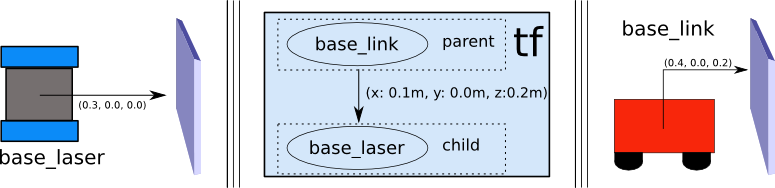
\includegraphics[width=0.5\textwidth,angle=0]{tutorials/tutorial_2/img/tf_robot.png}


\end{document}
